\documentclass{beamer}
\usetheme{Boadilla}
\usepackage{cmbright}
\setbeamertemplate{itemize items}[circle]
\setbeamertemplate{enumerate items}[default]

\title[Euler Equations]{Euler Equations and Money Market Interest Rates: \\ A Challenge for Monetary Policy Models}
\author[Canzoneri, Cumby \& Diba]{Matthew B. Canzoneri, Robert E. Cumby, and Behzad T. Diba
    Presented by Pearl Li}
\date{September 23, 2015}

\begin{document}

\begin{frame}
\titlepage
\end{frame}

\begin{frame}{Overview}
\begin{itemize}
\item Questions
\item Background
\item Data
\item Empirical Analysis
    \begin{itemize}
    \item Model
    \item Utility Specifications
    \end{itemize}
\item Results
\item Thesis Connection
\end{itemize}
\end{frame}

\begin{frame}{Questions}
\begin{itemize}
\item How do the interest rates implied by the consumption Euler equation compare to observed historical interest rates?
\item Is the spread between these two rates correlated with the stance of monetary policy?
\end{itemize}
\end{frame}

\begin{frame}{Background}
\begin{itemize}
\item Consumption Euler equation expresses intertemporal first-order condition
\item Typical form $u'(C_t) = \beta (1 + r_t) E_t u'(C_{t+1})$
\item Equivalently, $\frac{\beta E_t u'(C_{t+1})}{u'(C_t)} = \frac{1}{1+r_t}$ (i.e. MRS = MRT)
\item Households delay consumption when interest rates are high
\item \textbf{Assumption of nearly all standard macroeconomic models}
\end{itemize}
\end{frame}

\begin{frame}{Data}
\begin{itemize}
\item U.S. data from 1966-2004 (source unknown)
\item Quarterly time series for:
    \begin{enumerate}
    \item Money market interest rates
    \item Per capita consumption
    \item Inflation (log change in the deflator for nondurables and services consumption)
    \item Journal of Commerce industrial materials commodity price index
    \item Per capita real disposable income
    \item Federal funds rate
    \item Per capita real nonconsumption GDP
    \end{enumerate}
\end{itemize}
\end{frame}

\begin{frame}<1>[label=plan]{Empirical Analysis}
\begin{itemize}
\item<1,2-> {\color<3->{gray}Compute implied interest rates under 5 utility specifications}
\item<1,3-> {\color<4->{gray}Regress spread (model rate - observed rate) on 2 measures of monetary policy}
\item<1,4-> Estimate VAR of variables 2-7 on previous slide $$Y_t = A_0 + A_1 Y_{t-1} + \nu_t$$
\item<1,4-> Compute response of model rate to monetary policy shock under 2 sets of preferences and compare to impulse response of FFR
\end{itemize}
\end{frame}

\begin{frame}{Model}
\begin{itemize}
\item Representative agent maximizes lifetime utility $$u_t = \sum_{s=1}^\infty \beta^{s-t} E_t u(C_s, Z_s)$$ where $Z_s$ is the habit or reference level of consumption in period $s$
\item Real interest rate $r_t$ given by $$\frac{1}{1 + r_t} = \frac{\beta E_t u'(c_{t+1})}{u'(c_t)}$$
\end{itemize}
\end{frame}

\begin{frame}{Utility Specifications}
\begin{enumerate}
\item Standard, additively separable, constant relative risk aversion (CRRA): $u(C_t) = \frac{1}{1-\alpha} C_t^{1-\alpha}$
\item Fuhrer (2000): utility depends on ratio $\frac{C_t}{C_{t-1}^\gamma}$
\item  Christiano, Eichenbaum, \& Evans (2005): utility depends on difference $C_t - b C_{t-1}$
\item Abel (1990, 1999): utility depends on $\frac{C_t}{Z_t}$, where reference level $Z_t$ is aggregate consumption last period (external)
\item Campbell \& Cochrane (1999): utility depends on $C_t - Z_t$, where $Z_t$ is again external
\end{enumerate}
\end{frame}

\againframe<2>{plan}

\begin{frame}{Results}
\begin{center}
Computed Implied Rates
\end{center}
\resizebox{\textwidth}{!}{\begin{tabular}{|l|c||c|c|c|c|c|} \hline
    & & & & Christiano- & & \\
    & & & & Eichenbaum- &                 & Campbell- \\
    & Observed & CRRA & Fuhrer & Evans & Abel & Cochrane \\ \hline
Mean & 2.32 & 7.08 & 5.66 & 2.10 & 8.34 & 2.20 \\ \hline
Std Dev & 2.39 & 1.66 & 31.25 & 7.39 & 26.55 & 1.64 \\ \hline
Correlation & & -0.37 & -0.07 & -0.09 & -0.36 & -0.37 \\ \hline
\end{tabular}}
\bigskip
\begin{itemize}
\item Interest rates implied by Euler equation negatively correlated with observed historical rates
\item Negative correlation robust to specification of different utility functions
\item Effect is weaker for preferences that imply the Euler equation is extremely volatile
\end{itemize}
\end{frame}

\begin{frame}{Results}
\begin{columns}
\begin{column}{0.5\textwidth}
\begin{center}\resizebox{0.75\textwidth}{!}{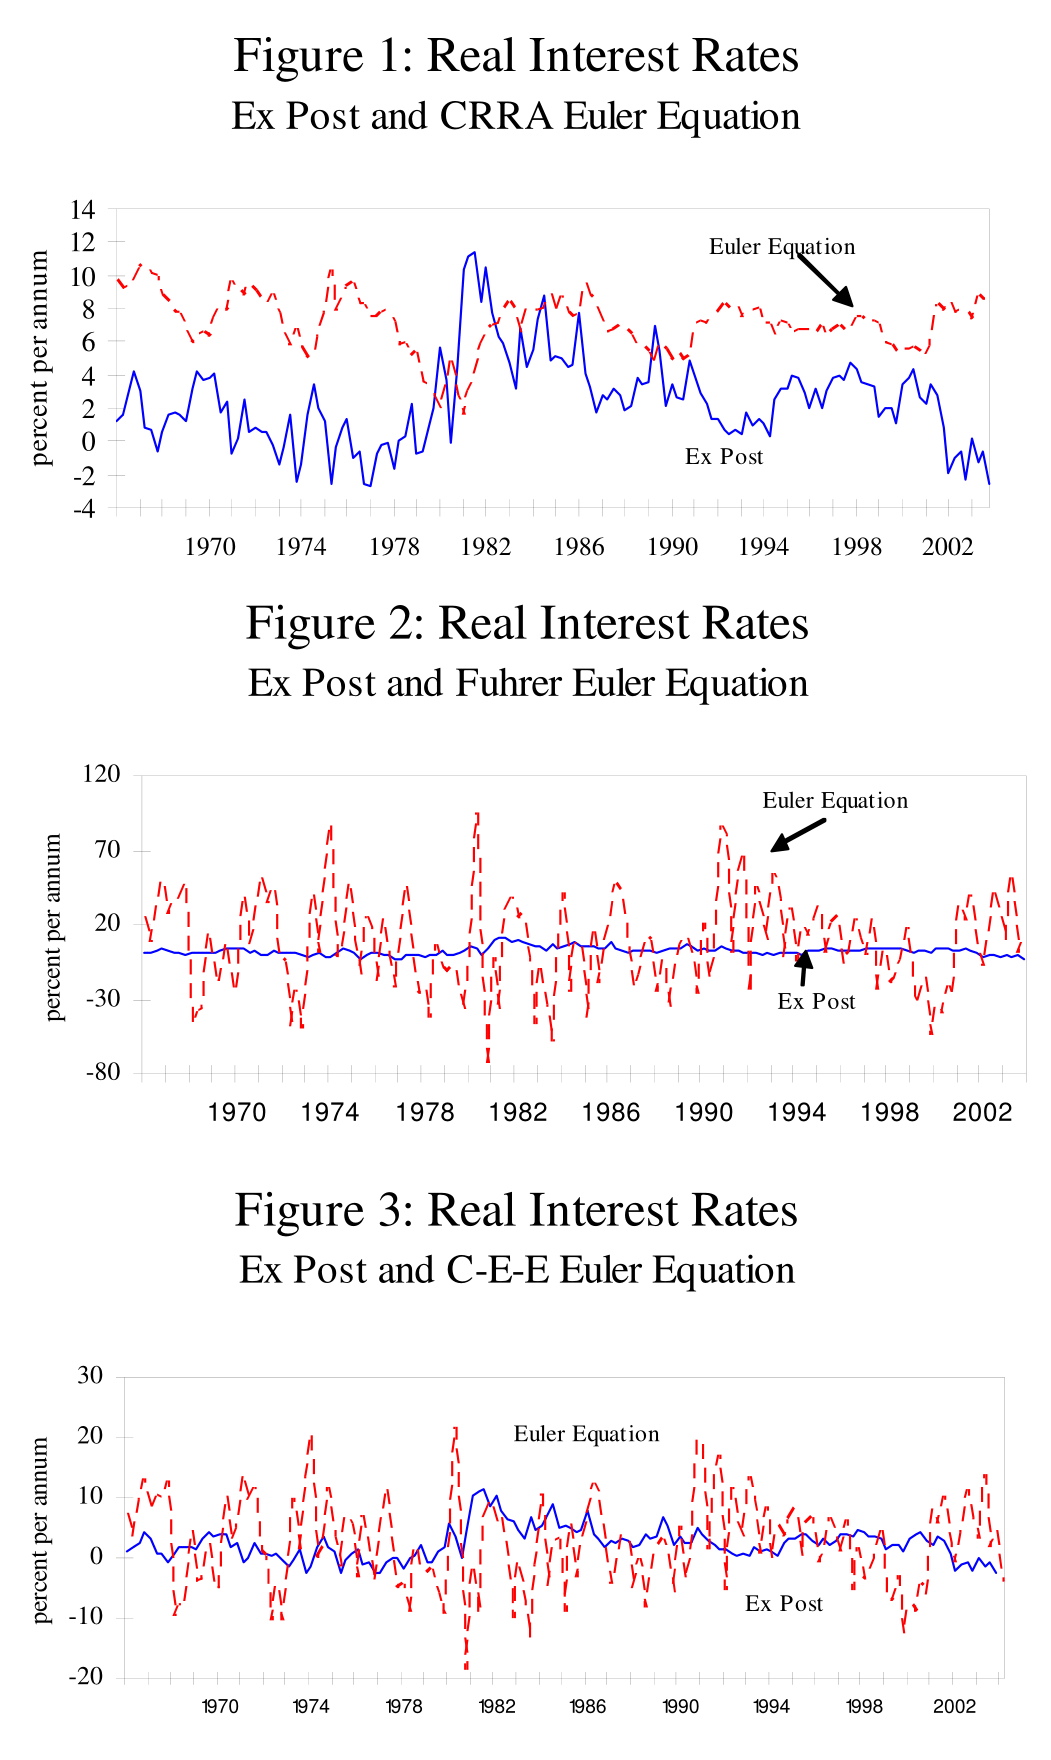
\includegraphics{figs1-3.png}}\end{center}
\end{column}
\begin{column}{0.5\textwidth}
\begin{center}\resizebox{0.75\textwidth}{!}{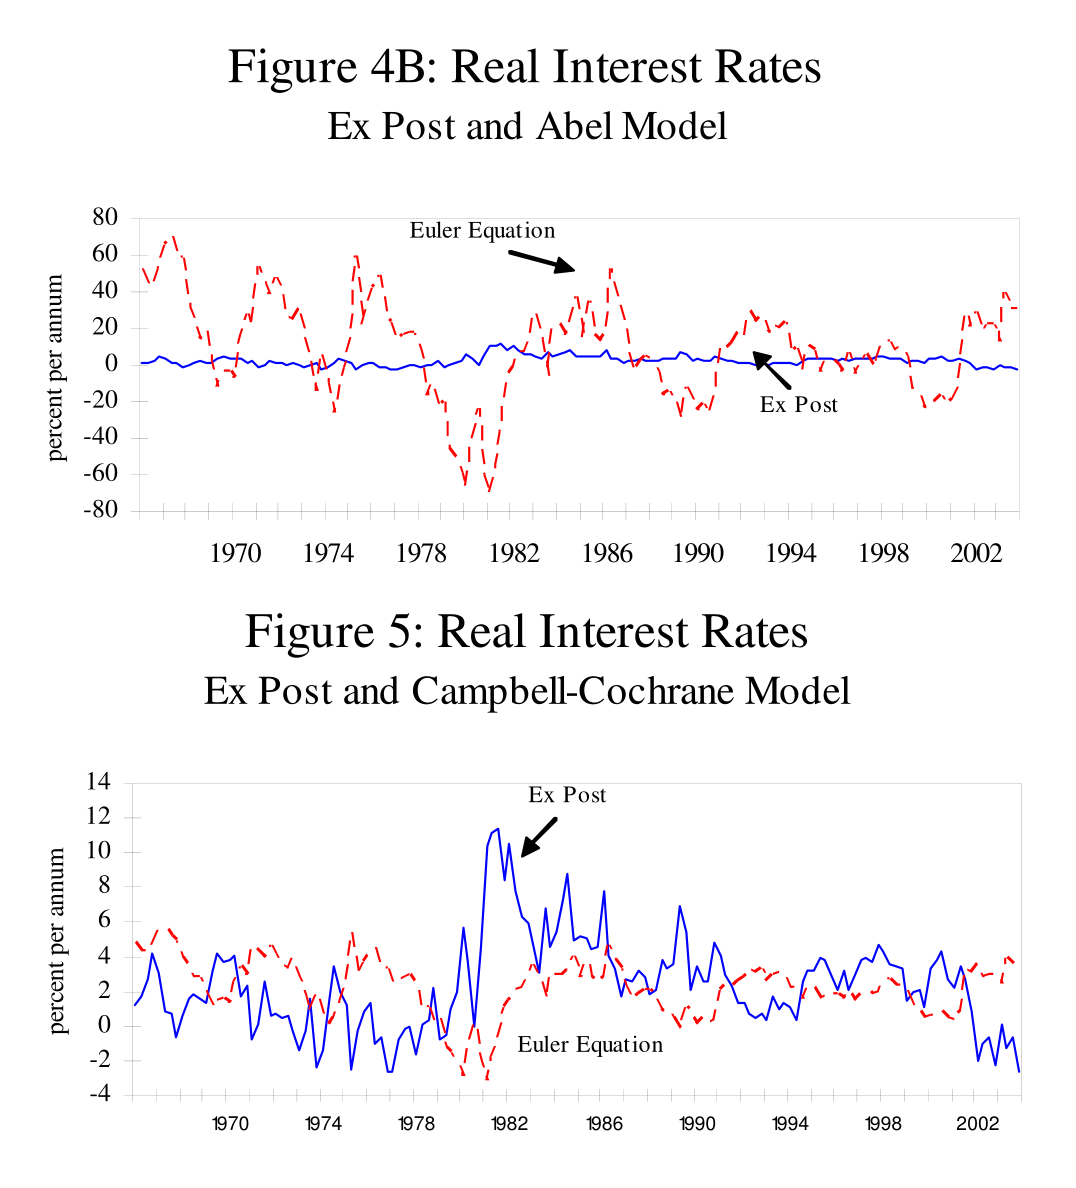
\includegraphics{figs4-5.png}}\end{center}
\end{column}
\end{columns}
\end{frame}

\againframe<3>{plan}

\begin{frame}{Results}
\begin{center}
Response of Interest Rate Spreads to Monetary Policy \\
(standard errors in parentheses)
\end{center}
\resizebox{\textwidth}{!}{\begin{tabular}{|l||c|c|c|c|c|} \hline
& & & Christiano- & & \\
& & & Eichenbaum- & & Campbell- \\
& CRRA & Fuhrer & Evans & Abel & Cochrane \\ \hline
FFR & -0.482 & -1.215 & -0.586 & -1.714 & -0.482 \\ 
    & (0.064) & (0.825) & (0.214) & (0.103) & (0.062) \\ \hline
S-Ratio & 0.062 & 0.263 & 0.079 & 0.346 & 0.015 \\
    & (0.015) & (0.214) & (0.052) & (0.103) & (0.015) \\ \hline
\end{tabular}}
\begin{itemize}
\item S-ratio = $\frac{\text{non-borrowed reserves } + \text{ extended credit}}{\text{total reserves}}$
\item Expansionary monetary policy (lower FFR, higher S-ratio) associated with significantly greater spreads
\end{itemize}
\end{frame}

\againframe<4>{plan}

\begin{frame}{Results}
\begin{center}
Impulse Response Functions for Federal Funds Rate Shock \\
\resizebox{0.75\textwidth}{!}{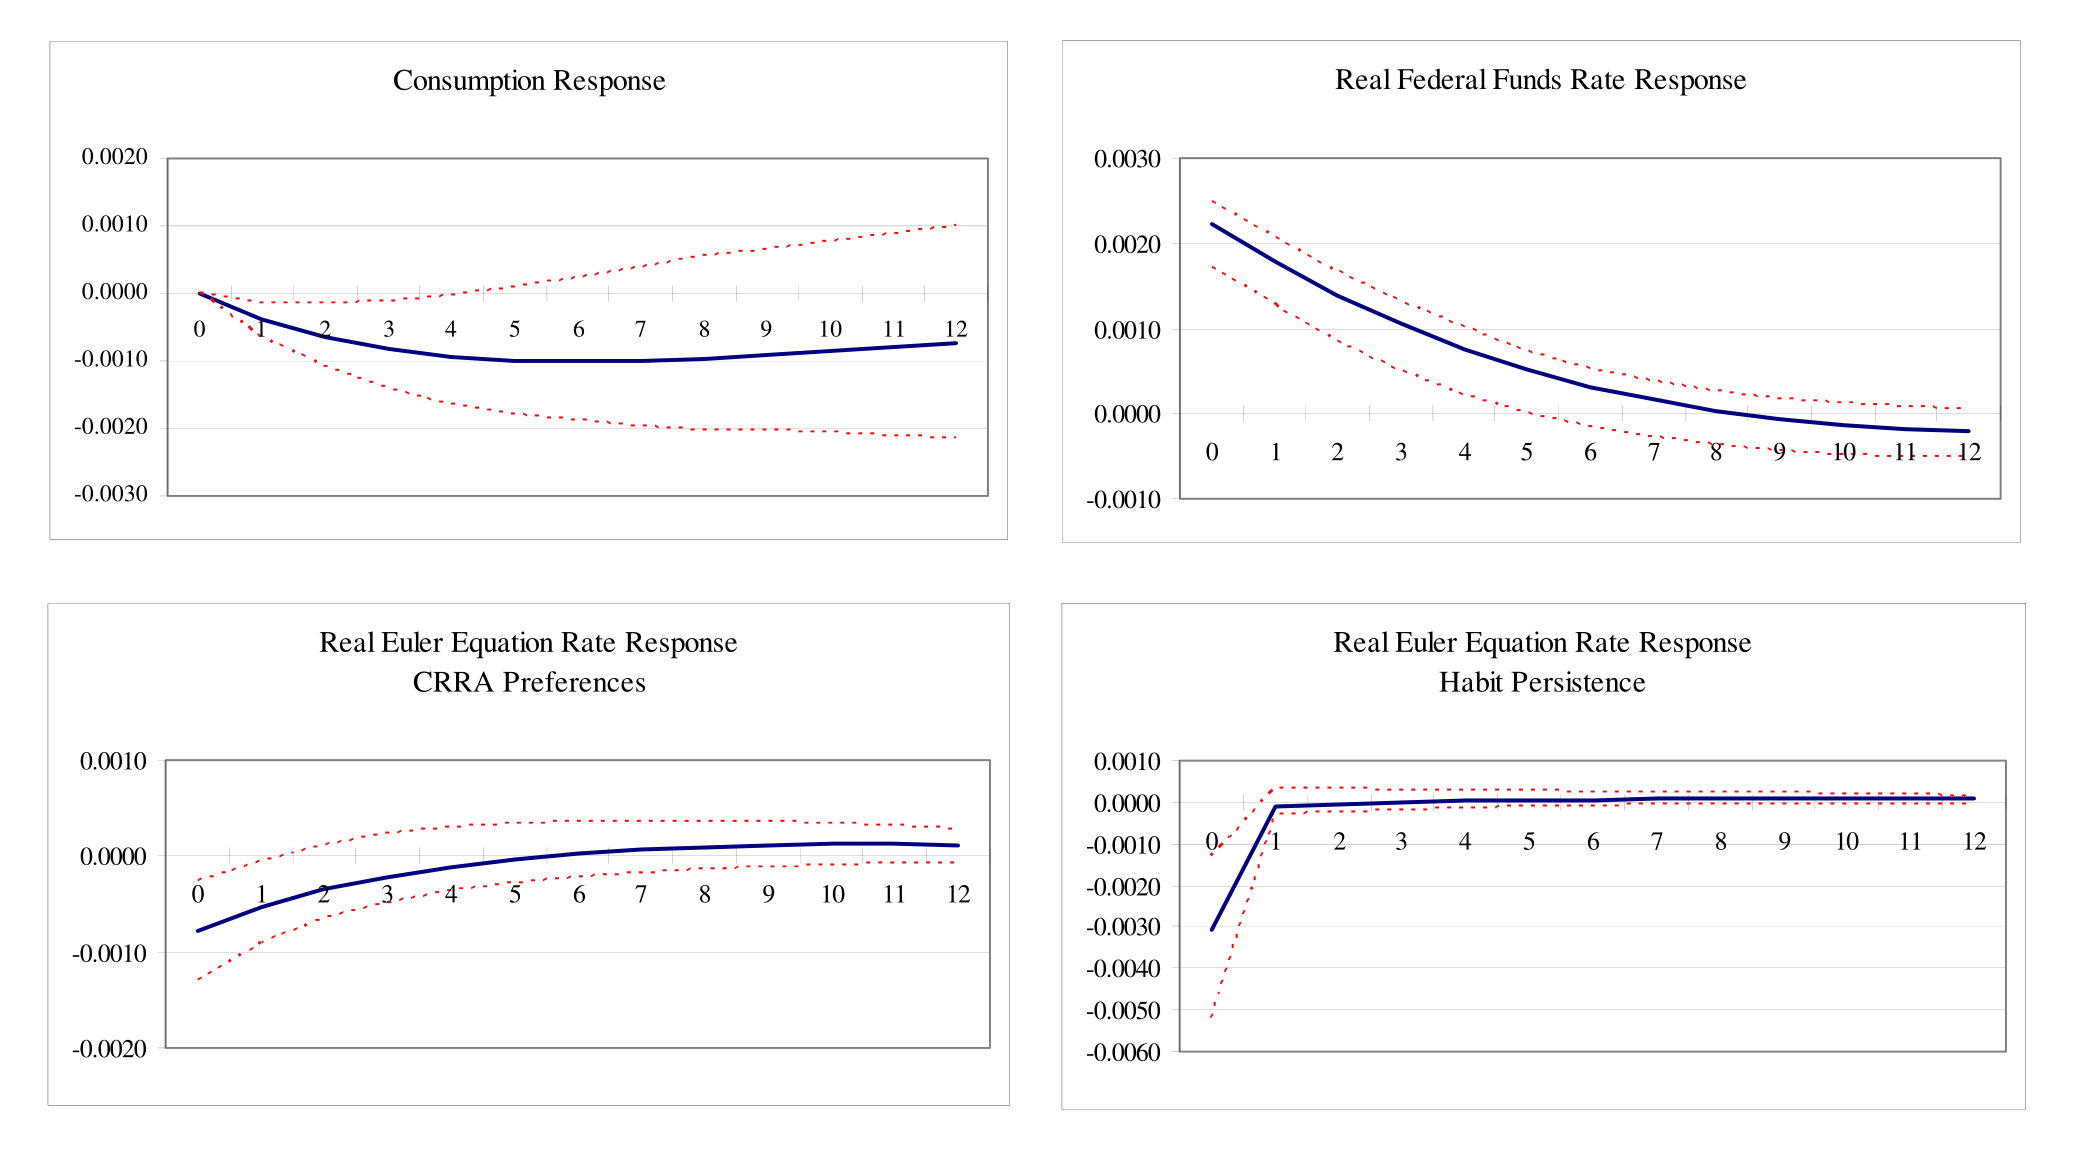
\includegraphics{fig6.png}}
\end{center}
\begin{itemize}
\item Euler equation rates and FFR move in opposite directions
\item Monetary tightening (raising FFR) decreases expected consumption growth, which is associated with decreasing real interest rates
\end{itemize}
\end{frame}

\begin{frame}{Thesis Connection}
\begin{itemize}
\item Want to test DSGE microfoundations, including consumption Euler equation
\item Rather than estimating system evolution with time series, will use closed-form solution of small-scale model
\end{itemize}
\end{frame}

\end{document}